\documentclass{beamer}
\usepackage[spanish]{babel}
\usepackage[utf8]{inputenc}
\usepackage{booktabs}
\usepackage{graphicx}

\usetheme{Berkeley}

\newcommand{\spaced}{\hspace{.2cm}}


\title{Filtrado de ruido en imágenes con transformada de wavelet}
\author{
  G.Isaias \and   
  M.Santiago \and 
  S.Lautaro Andres \and
  V.Xavier 
}
\institute{
  Universidad Nacional del Comahue \\ 
  Buenos Aires 14000, Neuquen \\ 
}
\date{}

\begin{document}
    
  \begin{frame}
    \titlepage  
  \end{frame}

  \begin{frame}
    \tableofcontents
  
    
  
  \end{frame}

  \section{Resumen}
\begin{frame}
\begin{block}{Resumen}
Los objetivos de esta presentación son:
\begin{itemize}
\item Dar una introducción a las funciones wavelets y transformada wavelet.
\item Estudiar y utilizar distintos umbrales para el filtrado de ruido.
\item Utilizar la transformada wavelet para filtrar ruido en imágenes.
\item Comparar este método de filtrado con otros.
\end{itemize}
\end{block}
\end{frame}

\section{Introducción}
\begin{frame}{Introducción a la transformada wavelet}
\begin{block}{Analogía con Fourier}

\begin{equation}
Fourier \rightarrow X(\omega) = \int_{-\infty}^{+\infty} x(t) e^{-j \omega t} dt
\end{equation}

\begin{equation}
 Wavelet \rightarrow X(a,b) = \int_{-\infty}^{+\infty} x(t) \overline{\psi_{a,b} (t)} dt
\end{equation}

\end{block}
\end{frame}

\begin{frame}

\begin{figure}
\centering
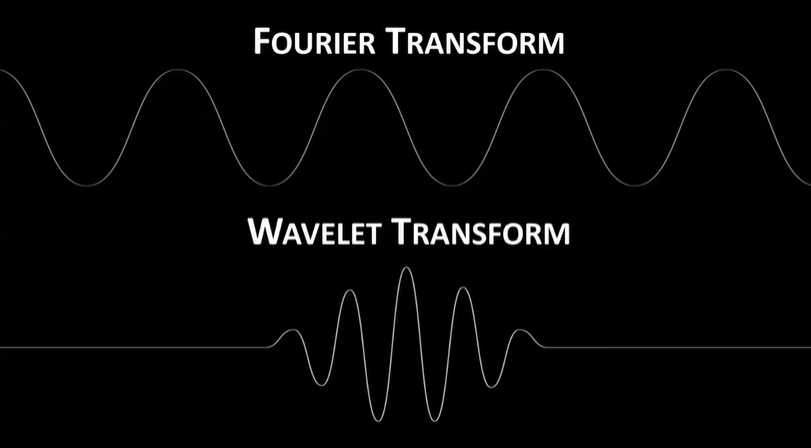
\includegraphics[width=\textwidth, height=6.5cm]{imgs/FvsW1}
\end{figure}

\end{frame}

\begin{frame}
\begin{figure}
\centering
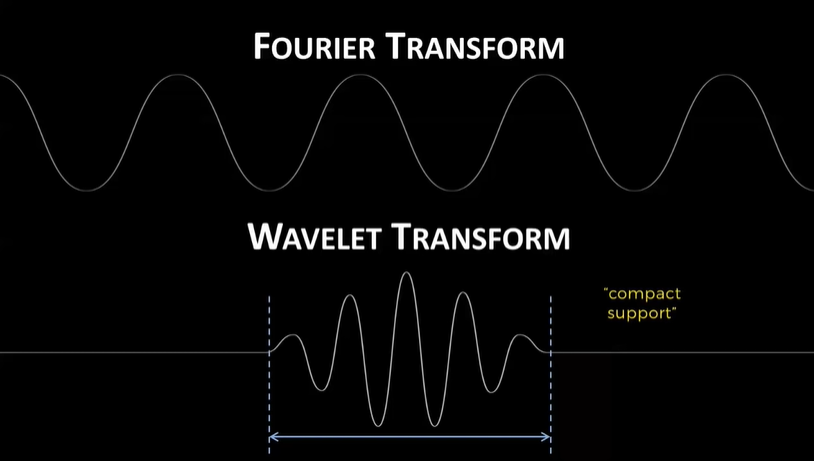
\includegraphics[width=\textwidth, height=6.5cm]{imgs/FvsW2}
\end{figure}
\end{frame}


\begin{frame}
\begin{figure}
\centering
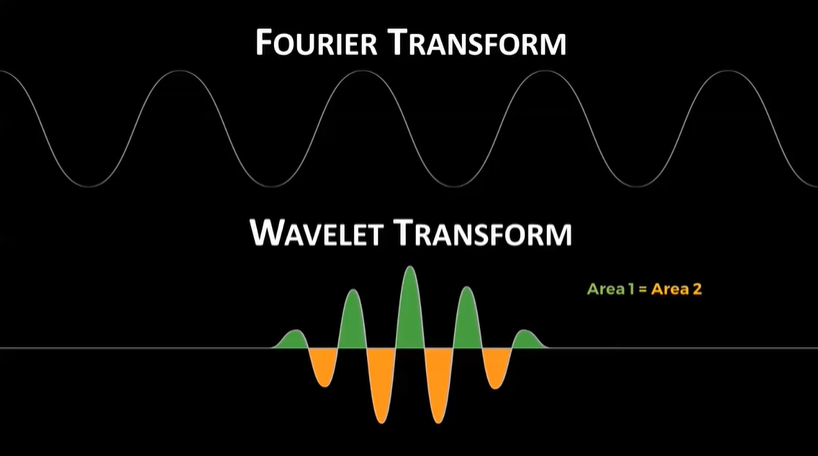
\includegraphics[width=\textwidth, height=6.5cm]{imgs/FvsW3}
\end{figure}
\end{frame}

\begin{frame}
\begin{figure}
\centering
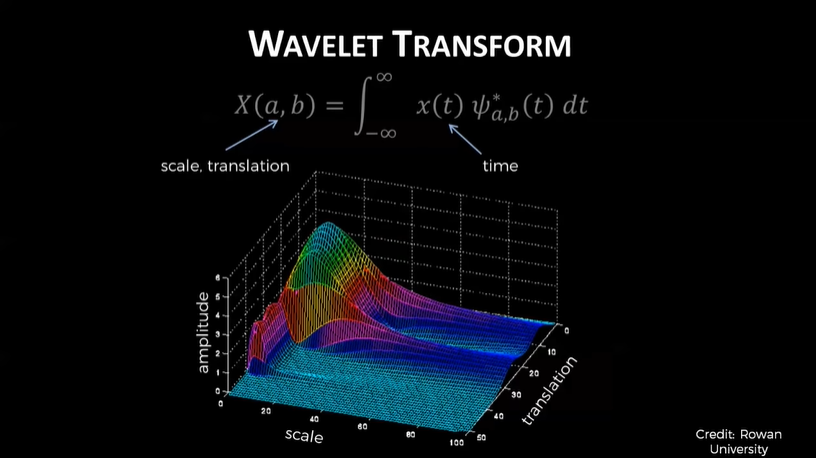
\includegraphics[width=\textwidth, height=6.5cm]{imgs/FvsW4}
\end{figure}
\end{frame}

\begin{frame}
\begin{figure}
\centering
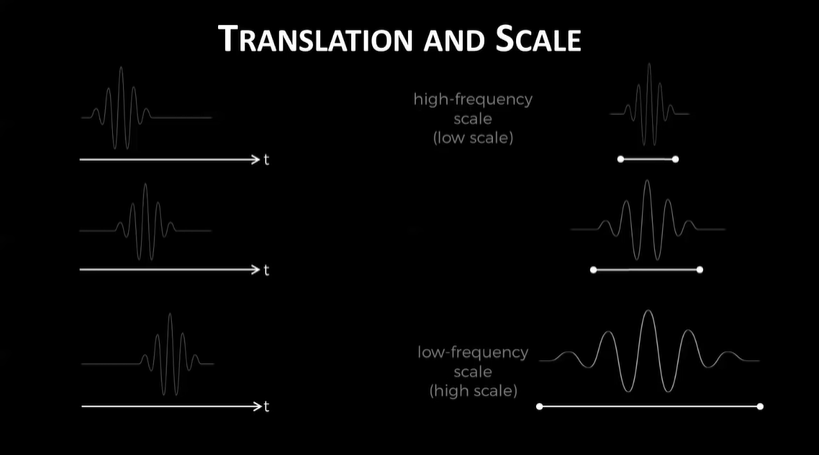
\includegraphics[width=\textwidth, height=6.5cm]{imgs/FvsW5}
\end{figure}
\end{frame}

\begin{frame}

\begin{block}{Matemáticamente...}
\begin{equation}
\psi_{a,b}(t)= \frac{1}{\sqrt{a}} \psi \left( \frac{t-b}{a} \right) \quad a,b \in \mathbb{R} \quad ; a \not = 0. 
\end{equation}


Si $a=2$ y $b=1$:

\begin{equation}
\psi_{j,k}(t) = 2^{-j/2} \psi (2^{-j} t-k )
\end{equation}

Las funciones $\{\psi_{j,k}\}_{\{j,k\} \in \mathbb Z }$ forman una base ortonormal de $L^2(\mathbb R)$.
\end{block}

\end{frame}
    

  \section{Marco Teórico}
  \subsection{Análisis multiresolución}
   
  
  \begin{frame}
   \frametitle{ Análisis multiresolución }
   Un análisis multiresolución para $L^{2}(\mathbb{R})$ consiste en una secuencia de subespacios cerrados de $L^{2}(\mathbb{R})$, $\{ V_{j} \}_{j \in \mathbb{Z} }$, una función  una función $\phi \in V_{0}$ tal que se cumplan las siguientes condiciones:

   \begin{itemize}
   \item[i.] Los espacios $V_{j}$ están anidados, es decir:
   \begin{equation*}
   ... \subset V_{-1} \subset V_{0} \subset V_{1} ...
   \end{equation*}
   \item[ii.] $\overline{\cup _{j\in \mathbb Z}V_j} = L^2(\mathbb R)$ y $\cap {j\in \mathbb Z}V_j = {0}$
   \item[iii.] Para todo $j \in \mathbb{Z}$, $V_{j-1}=D(V_j)$
   \item[iv.] $f \in V_0 \rightarrow T_kf \in V_o$, $\forall k \in \mathbb{Z}$
   \item[v.] $\{T_k \phi \}_{k \in \mathbb{Z}}$ es una base ortonormal de $V_0$
   \end{itemize} 
  \end{frame}
\begin{frame}
  \frametitle{Análisis multiresolución}
 Se define a $W_j$ como el complemento ortogonal de $V_j$ en $V_{j-1}$
  \begin{equation}
    \label{Central}
    V_{j-1} = V_j \oplus W_j
  \end{equation}
  \begin{equation}
    \label{NivApDet}
    A_{j-1}(t) = A_j(t) + D_j(t) 
  \end{equation} 
Por otro lado:
\begin{equation}
  V_J = V_K \oplus W_K \oplus ... \oplus W_{J+1}, \: J<K
  \label{eq.Vj}
  \end{equation}
Finalmente:
\begin{equation}
  x(t) = A_J(t) + \sum_{j=-\infty}^{J}D_j(t)
  \end{equation}

\end{frame}
\begin{frame}
\frametitle{Análisis multiresolución}
$\rightarrow$ Vemos ejemplo en el toolbox de Matlab
  
Para continuar:
\begin{itemize}
  \item 
  \begin{equation}
    A_j(t)=\sum_{k \in \mathbb Z} \beta _{j,k} \phi _{j,k}(t)
  \end{equation}
  Donde:
  \begin{equation}
    \label{Beta}
    \beta _{j,k}= <x(t), \phi _{j,k}(t)>
  \end{equation}

  \item
  \begin{equation}
    D_j(t)=\sum_{k \in \mathbb Z} \alpha _{j,k} \psi _{j,k}(t)
  \end{equation}
  Donde:
  \begin{equation}
    \label{Alfa}
    \alpha _{j,k}= <x(t), \psi _{j,k}(t)>
  \end{equation}
\end{itemize}
La función $\psi \in L^{2}(\mathbb{R})$ y $\{T_k \psi \}_{k \in \mathbb{Z}}$ son una base ortonormal de $W_0$
\end{frame}


\subsection{Banco de filtros}
  
  \begin{frame}
    \frametitle{¿Cómo solucionamos el inconveniente del producto interno?}
    
    Estrategia: Algoritmo que relacione las bases ortonormales y la idea de banco de filtros.
      
     Si partimos de la ecuación \ref{Central} y recordamos como se descomponían estas funciones, tenemos el inconveniente de los productos internos.
        
  \end{frame}

   \begin{frame}

Reescribiendo la ecuación \ref{Central} 
   \begin{equation}
\label{Aj}
A_j(t)=\sum_{k \in \mathbb Z}  a^{j}_{k} \phi _{j,k}(t)
\end{equation} 
\begin{equation}
\label{Dj}
D_j(t)=\sum_{k \in \mathbb Z}  d^{j}_{k} \psi _{j,k}(t)
\end{equation} 
con
\begin{equation}
\label{ajk}
a^{j}_{k}= <A_{j}(t), \phi _{j,k}(t)>
\end{equation}
\begin{equation}
\label{ajk}
d^{j}_{k}= <A_{j}(t), \psi _{j,k}(t)>
\end{equation}
    \end{frame}
    
  \begin{frame}
   Podemos obtener $a^{j}$y $d^{j}$ a partir de $A_{j-1}$, partiendo del producto interno de $A_{j-1}$ y las funciones de escala y wavelet
   \begin{equation}
<A_{j-1}(t),\psi _{j,k}(t)>=<A_{j}(t)+D_{j},\psi _{j,k}(t)>
\end{equation}

\begin{equation}
<A_{j-1}(t),\phi _{j,k}(t)>=<A_{j}(t)+D_{j},\phi _{j,k}(t)>
\end{equation}
  \end{frame}
  
  \begin{frame}
  A su ves sabemos que:
  
  \begin{equation}
  A_{j-1}(t)=\sum_{k \in \mathbb{Z}} a^{j-1}_{k} \phi^{j-1}_{k}(t)
  \end{equation}
  
  con lo que obtenemos que: 
  
  \begin{equation}
  a^{j}_{k}=\sum_{p \in \mathbb{Z}} a^{j-1}_{p} <\phi_{j-1,p},\phi_{j,k}>
  \end{equation}
  
  \begin{equation}
  d^{j}_{k}=\sum_{p \in \mathbb{Z}} a^{j-1}_{p} <\phi_{j-1,p},\psi_{j,k}>
  \end{equation}
  \end{frame}
  
  \begin{frame}
  Pero tanto los productos internos de $<\phi_{j-1,p},\phi_{j,k}>$ $<\phi_{j-1,p},\psi_{j,k}>$, son productos internos de funciones conocidas que ya fueron calculadas por lo cual podríamos tomarlo como coeficientes conocidos más aún como coeficientes de filtros.
  
\begin{equation}
	\sqrt{2} a_{p-2k}=<\phi _{j-1,p}(t),\phi _{j,k}(t)>
\end{equation}
	
\begin{equation}
	\sqrt{2} b_{p-2k}=<\phi _{j-1,p}(t),\psi _{j,k}(t)>
\end{equation}
  
  \end{frame}
\begin{frame}
Por lo que se definen los coeficientes de los filtros 
\begin{equation}
[LD]_{n}=\sqrt{2}  a_{-n}
\end{equation}

\begin{equation}
[HD]_{n}=\sqrt{2}  b_{-n}
\end{equation}
Donde LD es un filtro pasa bajos y HD es un filtro pasa altos.
Por lo que reescribimos a $a^{j}_k$ y $d^{j}_k$
\begin{equation}
\label{afinal}
a^{j}_{k}=\sum_{p \in \mathbb Z} a^{j-1}_{p} [LD]_{2k-p}
\end{equation}

\begin{equation}
\label{dfinal}
d^{j}_{k}=\sum_{p \in \mathbb Z} a^{j-1}_{p} [HD]_{2k-p}
\end{equation}

\end{frame}
\begin{frame}
Gráficamente lo visualizamos

\begin{figure}[htb]
	\centering
	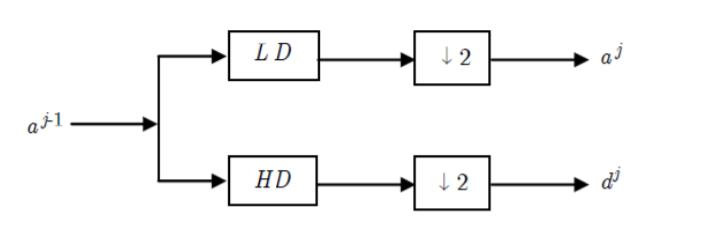
\includegraphics[width=.75\textwidth]{imgs/bancofiltros1D}
	\caption{Descomposición con banco de filtros para 1D.}
	\label{bancofiltros1D}
\end{figure}
\end{frame}
\begin{frame}
Para el caso de imágenes, la descomposición en 2D se ve como un doble filtrado
\begin{figure}[H]
	\centering
	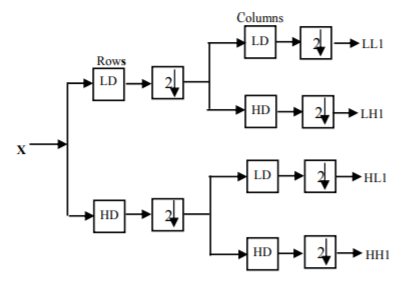
\includegraphics[width=.75\textwidth]{imgs/bancofiltros}
	\caption{Descomposición con banco de filtros para 2D.}
	\label{bancofiltros}
\end{figure}
\end{frame}
\begin{frame}
Es posible realizar el proceso inverso y recuperar la señal original
\begin{figure}[H]
	\centering
	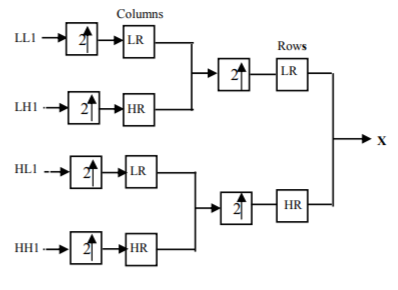
\includegraphics[width=.75\textwidth]{imgs/bancofiltrosR}
	\caption{Recomposición con banco de filtros para 2D.}
	\label{bancofiltrosR}
\end{figure}
\end{frame}

\begin{frame}
\subsection{Umbralización}
\frametitle{Umbralización}
\centering
\begin{figure}[htb]
  \centering
  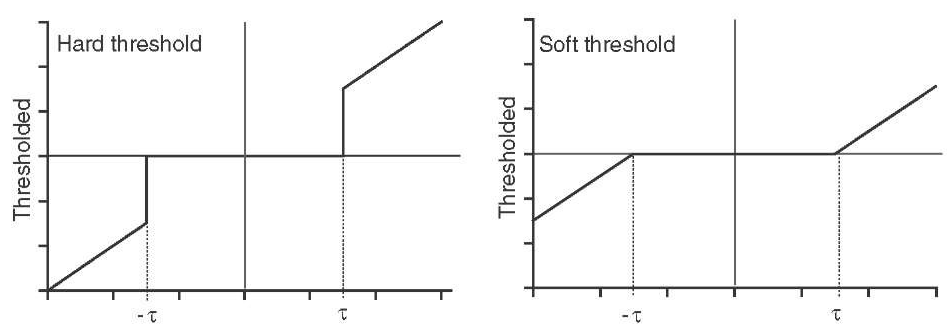
\includegraphics[scale=0.4]{imgs/Umbral}
  \caption{Modos de umbralización más utilizados}
  \label{}
\end{figure}
\end{frame}

\begin{frame}
  \frametitle{Umbralización}
Algoritmos para el cálculo del umbral $\tau$:
\begin{itemize}
  \item VisuShrink
  \item LevelShrink
  \item BayesShrink
  \item NormalShrink
  \item AWT(Adaptative Wavelet Treshholding)
\end{itemize}
\end{frame}






  \section{Implementación}

  \begin{frame}
    \frametitle{Pseudocódigo parámetros óptimos}
  
    \begin{itemize}
      \item Leer todas las imágenes de una carpeta y normalizar sus valores entre 0 y 1.
      \item Agregar ruido gaussiano con $\mu=0$ y varianza $\sigma$.
      \item Seleccionar el parámetro a variar, y dejar constante el resto de parámetros.
      \item Transformar la imagen utilizando la transformada de wavelet.
      \item Calcular los umbrales para cada nivel segun el umbral seleccionado.
      \item Aplicar el modo (soft - hard) y eliminar las componentes menores al umbral.
      \item Aplicar la antitransformada.
      \item Calcular el PSNR y el SSIM.
    \end{itemize}
  
  \end{frame}

  \section{Resultados}

  \subsection{Imágenes de prueba}

  \begin{frame}
    \frametitle{ Lenna - $\sigma=0.3$ }
    \centering
    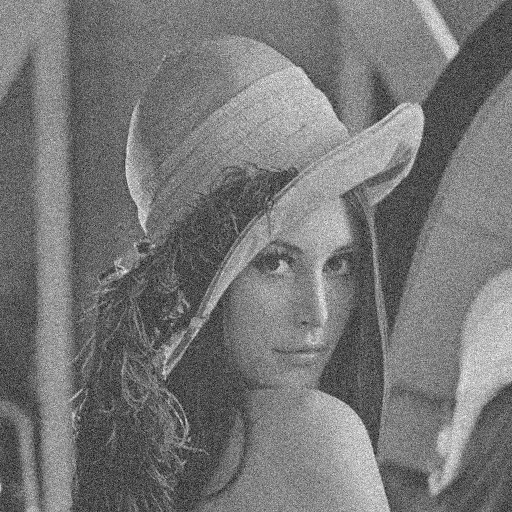
\includegraphics[width=5cm]{imgs/Noise/Lenna.jpg}
  \end{frame}

  \begin{frame}
    \frametitle{ House - $\sigma=0.3$ }  
    \centering
    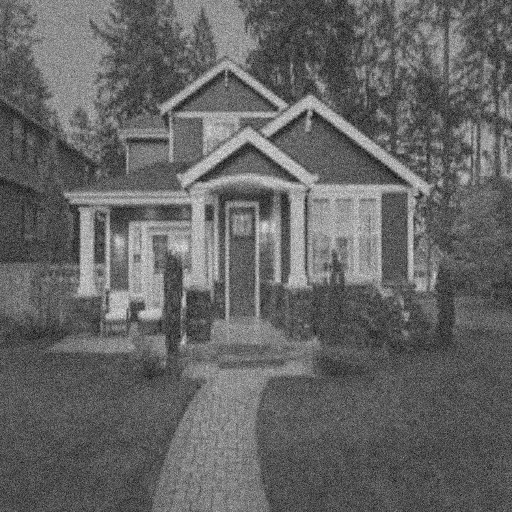
\includegraphics[width=5cm]{imgs/Noise/House.jpg}
  \end{frame}

  \begin{frame}
    \frametitle{ Wave - $\sigma=0.3$ }
    \centering
    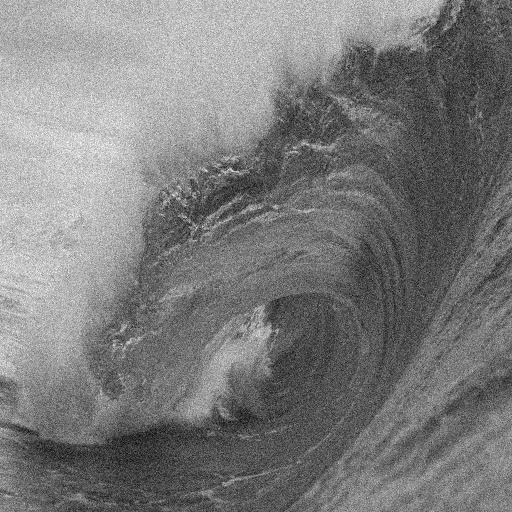
\includegraphics[width=5cm]{imgs/Noise/Wave.jpg}
  \end{frame}

  \subsection{Parámetros óptimos}

  \begin{frame}
    \frametitle{ Comparación de Niveles }
    \centering
    \begin{tabular}{lrrrrr}
      \toprule
      {PSNR} &  noise &      1 &      2 &      4 &      6 \\
      \midrule
      Lenna &  17.65 &  23.92 &  \bf{27.03} &  22.29 &  22.29 \\
      House &  19.87 &  22.90 &  \bf{25.58} &  24.57 &  23.51 \\
      Wave &  18.63 &  23.34 &  \bf{26.70} &  24.71 &  24.65 \\
      \bottomrule
      \end{tabular}
  
      \begin{tabular}{lrrrrr}
        {SSIM} &  noise &      1 &      2 &      4 &      6 \\
        \midrule
        Lenna &  0.518 &  0.742 &  \bf{0.856} &  0.847 &  0.808 \\
        House &  0.620 &  0.806 &  \bf{0.882} &  0.839 &  0.814 \\
        Wave &  0.586 &  0.761 &  \bf{0.839} &  0.820 &  0.803 \\
        \bottomrule
        \end{tabular}

  \end{frame}

  \begin{frame}
    \frametitle{ Comparación de Niveles }
    \centering
    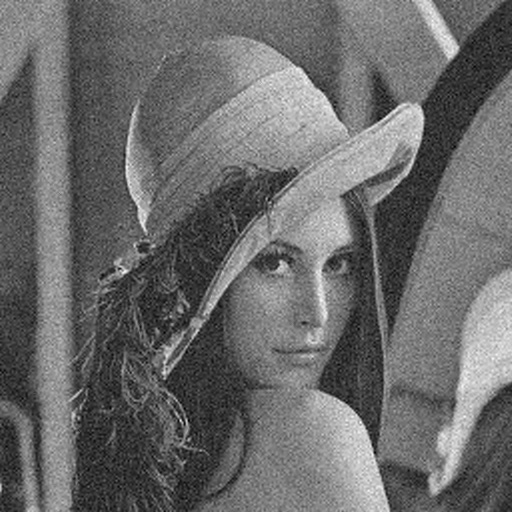
\includegraphics[width=3.5cm]{imgs/Levels/1_normal_soft_sym8_Lenna.jpg}
    \spaced
    \includegraphics[width=3.5cm]{imgs/Levels/2_normal_soft_sym8_Lenna.jpg}
    \\
    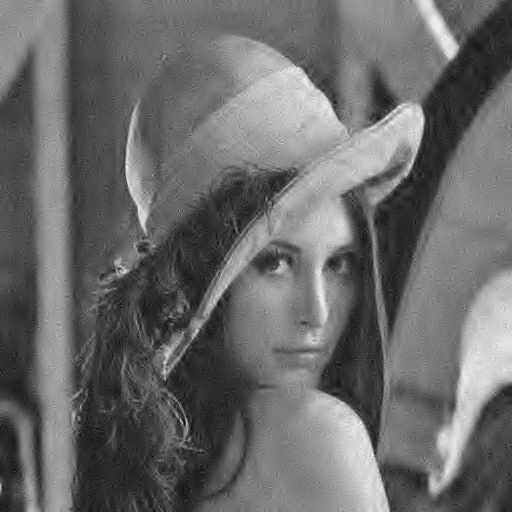
\includegraphics[width=3.5cm]{imgs/Levels/4_normal_soft_sym8_Lenna.jpg}
    \spaced
    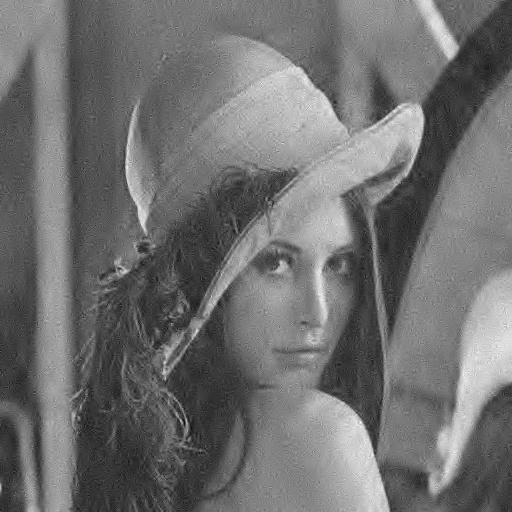
\includegraphics[width=3.5cm]{imgs/Levels/6_normal_soft_sym8_Lenna.jpg}
  
  \end{frame}

  \begin{frame}
    \frametitle{Comparación de niveles 2 - 6}
    \centering
    \includegraphics[width=5cm]{imgs/Levels/2_normal_soft_sym8_Lenna.jpg}  
    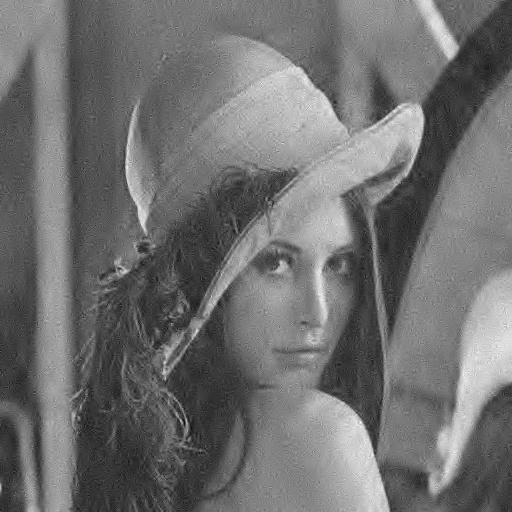
\includegraphics[width=5cm]{imgs/Levels/6_normal_soft_sym8_Lenna.jpg}
  
  \end{frame}

  \begin{frame}
    \frametitle{ Comparación de modos }
    \centering
    \begin{tabular}{lrrr}
      \toprule
      {PSNR} &  noise &   soft &   hard \\
      \midrule
      Lenna &  17.65 &  \bf{27.03} &  21.41 \\
      House &  19.87 &  \bf{25.58} &  20.20 \\
      Wave &  18.63 &  \bf{26.70} &  20.85 \\
      \bottomrule
      \end{tabular}
      \begin{tabular}{lrrr}
        {SSIM} &  noise &   soft &   hard \\
        \midrule
        Lenna &  0.518 &  \bf{0.856} &  0.757 \\
        House &  0.620 &  \bf{0.882} &  0.789 \\
        Wave &  0.586 &  \bf{0.839} &  0.755 \\
        \bottomrule
        \end{tabular}

  \end{frame}

  \begin{frame}
    \frametitle{ Comparación de modos }
    \centering
    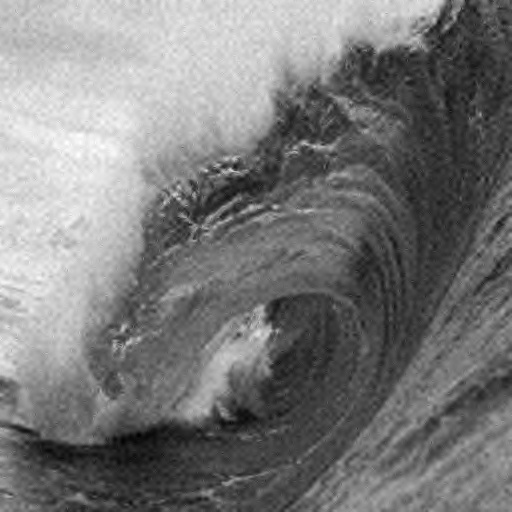
\includegraphics[width=5cm]{imgs/Modes/2_normal_soft_sym8_Wave.jpg}
    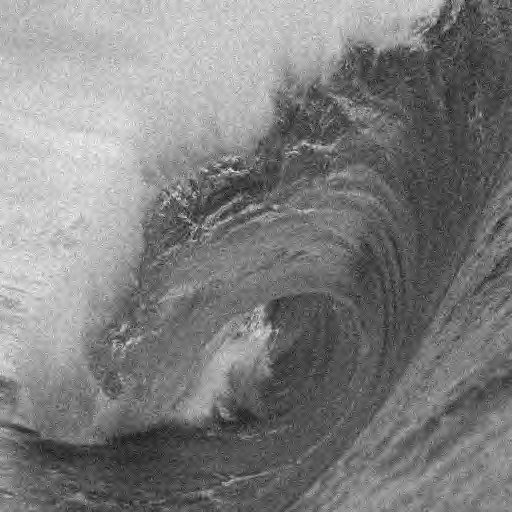
\includegraphics[width=5cm]{imgs/Modes/2_normal_hard_sym8_Wave.jpg}

  \end{frame}

  \begin{frame}
    \frametitle{ Comparación de umbrales }
    \centering
    \begin{tabular}{lrrrrrr}
      \toprule
      {PSNR} &  noise &  universal &  bayes &  level &  normal &    awt \\
      \midrule
      Lenna &  17.65 &      25.86 &  25.71 &  25.40 &   \bf{27.03} &  25.24 \\
      House &  19.87 &      22.91 &  23.32 &  23.19 &   \bf{25.58} &  23.41 \\
      Wave &  18.63 &      26.74 &  26.70 &  \bf{26.86} &   26.70 &  25.56 \\
      \bottomrule
      \end{tabular}
      \begin{tabular}{lrrrrrr}
        {SSIM} &  noise &  universal &  bayes &  level &  normal &    awt \\
        \midrule
        Lenna &  0.518 &   0.848 &  0.847 &  0.849 &  \bf{0.856} &  0.838 \\
        House &  0.620 &   0.851 &  0.850 &  0.857 &  \bf{0.882} &  0.849 \\
        Wave &  0.586 &   0.830 &  0.829 &  0.833 &  \bf{0.839} &  0.823 \\
        \bottomrule
        \end{tabular}



  \end{frame}

  \begin{frame}
    \frametitle{ Comparación de umbrales }
  
    \centering
    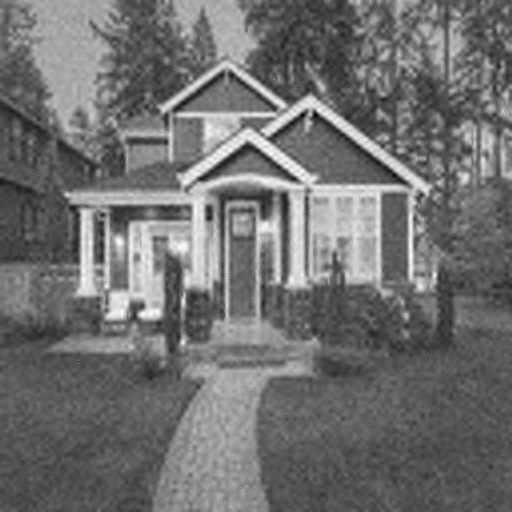
\includegraphics[width=3cm]{imgs/Thresholds/2_awt_soft_sym8_House.jpg}
    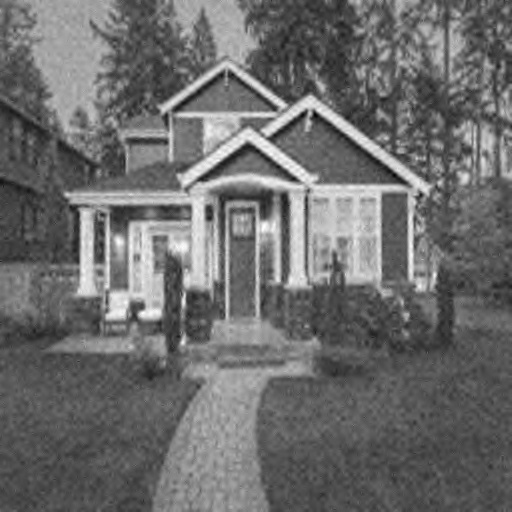
\includegraphics[width=3cm]{imgs/Thresholds/2_normal_soft_sym8_House.jpg}
    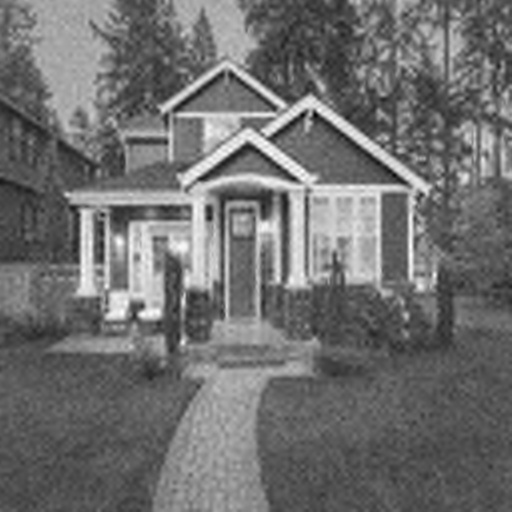
\includegraphics[width=3cm]{imgs/Thresholds/2_universal_soft_sym8_House.jpg}
    \\
    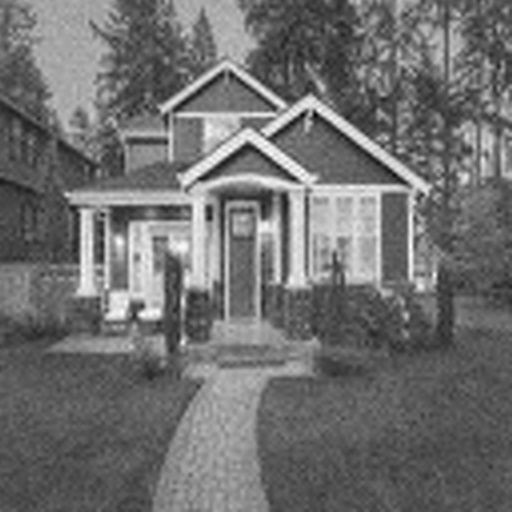
\includegraphics[width=3cm]{imgs/Thresholds/2_bayes_soft_sym8_House.jpg}
    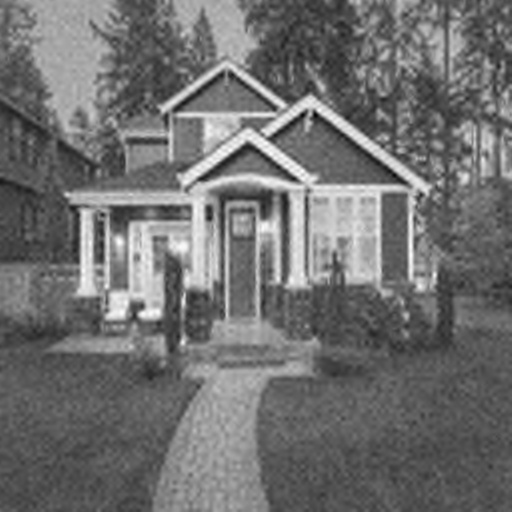
\includegraphics[width=3cm]{imgs/Thresholds/2_level_soft_sym8_House.jpg}
    

  \end{frame}

  \begin{frame}
    \frametitle{Comparación de la wavelet madre}
    \centering
    \begin{tabular}{lrrrr}
      \toprule
      {PSNR} &  noise &   haar &    db4 &   sym8 \\
      \midrule
      Lenna &  17.65 &  23.44 & 25.19 &  \bf{27.03} \\
      House &  19.87 &  \bf{26.38} &  24.78 &  25.58 \\
      Wave &  18.63 &  24.67 &  \bf{26.87} &  26.70 \\
      \bottomrule
      \end{tabular}
  
      \begin{tabular}{lrrrr}
        {SSIM} &  noise &   haar &    db4 &   sym8 \\
        \midrule
        Lenna &  0.518 &  0.819 &  0.853 &  \bf{0.856} \\
        House &  0.620 &  0.848 &  0.875 &  \bf{0.882} \\
        Wave &  0.586 &  0.805 &  0.836 &  \bf{0.839} \\
        \bottomrule
        \end{tabular}
  \end{frame}

  \begin{frame}
    \frametitle{Comparación de la wavelet madre - db4}
    
    \centering
    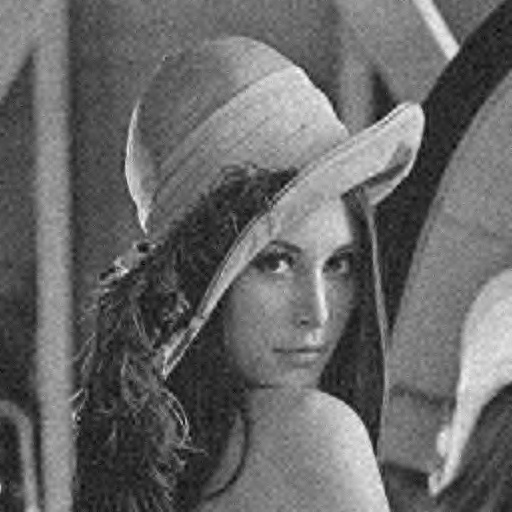
\includegraphics[width=6cm]{imgs/Wavelets/2_normal_soft_db4_Lenna.jpg}
   
  
  \end{frame}

  \begin{frame}
    \frametitle{Comparación de la wavelet madre - haar}
    
    \centering
    
    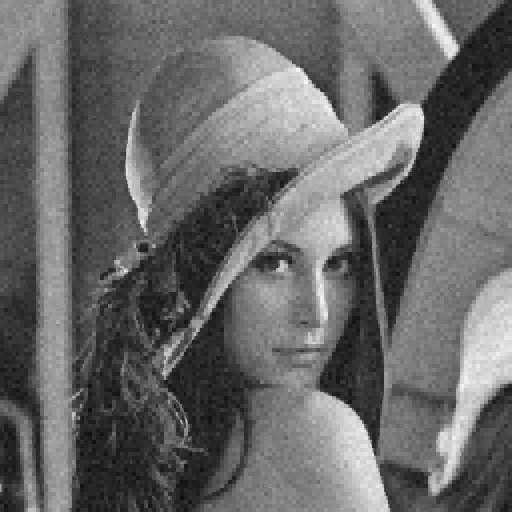
\includegraphics[width=6cm]{imgs/Wavelets/2_normal_soft_haar_Lenna.jpg}
    

  
  \end{frame}

  \begin{frame}
    \frametitle{Comparación de la wavelet madre - sym8}
    
    \centering
    
    
    \includegraphics[width=6cm]{imgs/Wavelets/2_normal_soft_sym8_Lenna.jpg}

  
  \end{frame}

  \begin{frame}
    \frametitle{Parámetros óptimos}
    \centering
    \begin{tabular}{llll}
      \toprule
      level & wavelet & mode & umbral \\
      \midrule 
      6 & sym8 & soft & normal \\
      \bottomrule
    \end{tabular}
  
  \end{frame}

  \subsection{Comparación de filtros}

  \begin{frame}
    \frametitle{Resultado del filtrado}
    \centering
    \begin{tabular}{lrrrr}
      \toprule
      {} &  noise &  wavelet &  wiener &  gaussian \\
      \midrule
      Lenna &  23.10 &    23.83 &   \bf{26.30} &     26.14 \\
      House &  24.80 &    25.07 &   \bf{28.28} &     27.99 \\
      Wave &  24.21 &    24.33 &   \bf{27.00} &     26.86 \\
      \bottomrule
      \end{tabular}
    
  
    \begin{tabular}{lrrrr}
      { SSIM } &  noise &  wavelet &  wiener &  gaussian \\
      \midrule
      Lenna &  0.647 &  \bf{0.870} &  0.843 &  0.835 \\
      House &  0.740 &  \bf{0.906} &  0.895 &  0.886 \\
      Wave &  0.693 &  \bf{0.887} &  0.862 &  0.853 \\
      \bottomrule
      \end{tabular}
  \end{frame}

  \begin{frame}
    \frametitle{Wavelet}
    \centering
    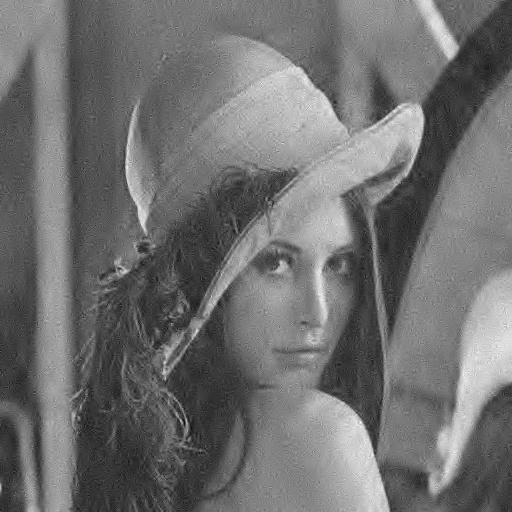
\includegraphics[width=6cm]{imgs/Comparacion/wavelet_Lenna.jpg}
  
  \end{frame}

  \begin{frame}
    \frametitle{Wiener}
  
    \centering

    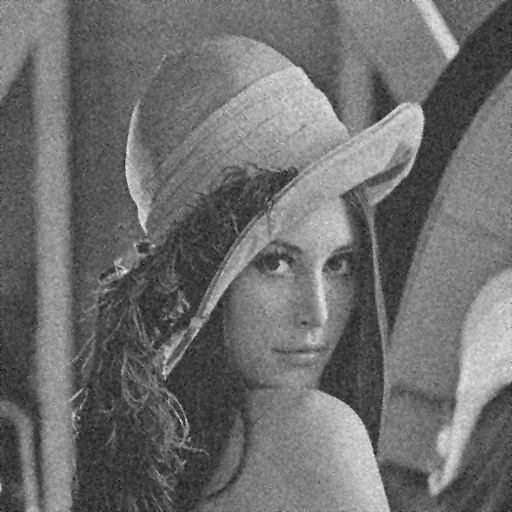
\includegraphics[width=6cm]{imgs/Comparacion/wiener_Lenna.jpg}
  
  \end{frame}


  \begin{frame}
    \frametitle{Gaussiano}
  
    \centering
    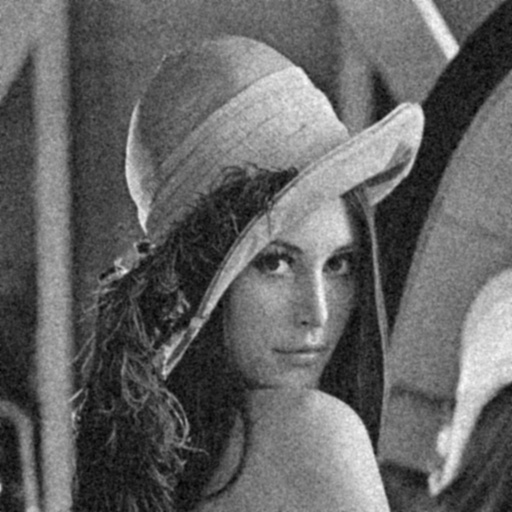
\includegraphics[width=6cm]{imgs/Comparacion/gaussian_Lenna.jpg}
  
  \end{frame}

  \subsection{Imágenes reales}

  \begin{frame}
    \frametitle{Principe de gales - 1925}
    \centering
    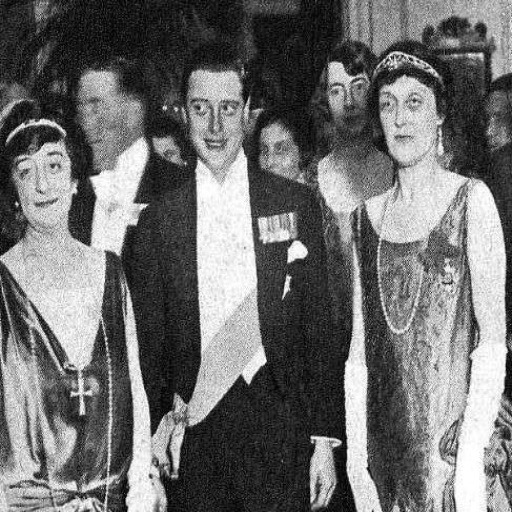
\includegraphics[width=5cm]{imgs/Real-resize/1.jpg}
    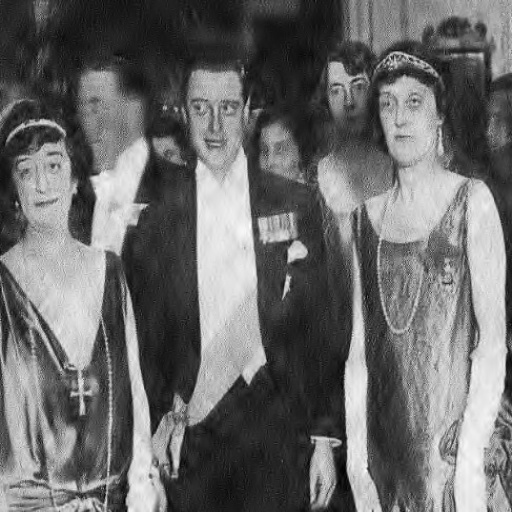
\includegraphics[width=5cm]{imgs/Real/1.jpg}
   
  \end{frame}

  \begin{frame}
    \frametitle{Resonancia magnética}
    \centering
    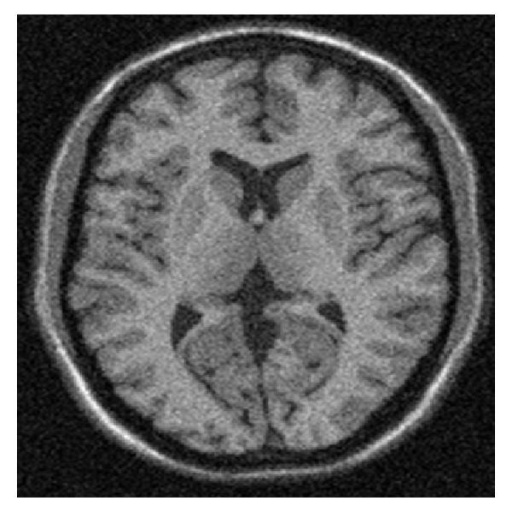
\includegraphics[width=5cm]{imgs/Real-resize/0.jpg}
    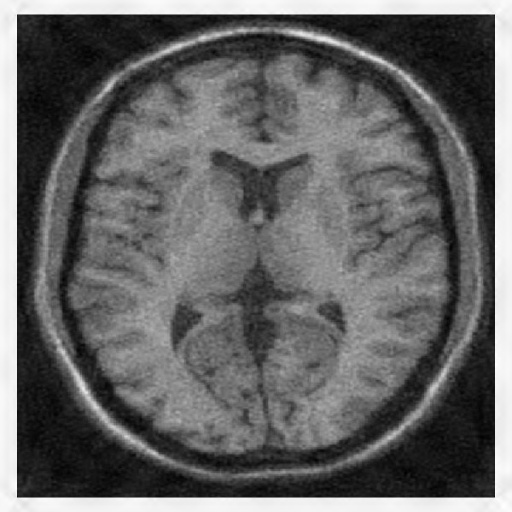
\includegraphics[width=5cm]{imgs/Real/0.jpg}  
  \end{frame}

  \section{Conclusiones}

\end{document}
